\documentclass[aspectratio=169]{beamer}
\usetheme{metropolis}

\usepackage{graphicx}
\usepackage{booktabs}
\usepackage{tabularx}
\usepackage{hyperref}
\usepackage{xcolor}

\title{What Do AI Agents Actually Change?}
\subtitle{An Empirical Taxonomy of Mutation Patterns\\in Performance-Improving Pull Requests}
\date{SSBSE 2026 Challenge}
\author[I. Dovhoshliubnyi et al.]{Illia Dovhoshliubnyi\inst{1} \and
        Nima Soroush\inst{1} \and
        Ashkan Sami\inst{1} \and
        Alexander Brownlee\inst{2}}
\institute{
  \inst{1}Edinburgh Napier University, Edinburgh, UK \\
  \texttt{illiadovho@gmail.com}, \texttt{\{N.Soroush, A.Sami\}@napier.ac.uk}
  \and
  \inst{2}University of Stirling, Stirling, UK \\
  \texttt{alexander.brownlee@stir.ac.uk}
}

\begin{document}

\maketitle

%---------------------------------------------------------
\begin{frame}{AI Coding Agents: The Black Box}
  \begin{itemize}
    \item \textbf{Autonomous Diffs}: Agents (Devin, Copilot, Cursor, Codex, Claude Code) submit PRs at scale, but their decision processes are proprietary and opaque.
    \item \textbf{The Diffs Speak}: We can't see \emph{how} they think, but we can inspect \emph{what} they change.
    \item \textbf{Our Goal}: Analyze successful performance-improving PRs from these agents to reverse-engineer their mutation behavior.
  \end{itemize}
\end{frame}

%---------------------------------------------------------
\begin{frame}{Why This Matters for SBSE \& GI}
  \begin{itemize}
    \item \textbf{Empirical Operators}: Genetic Improvement (GI) and Search-Based Software Engineering (SBSE) rely on mutation operators reflecting real-world changes.
    \item \textbf{The Gap}: Current taxonomies are derived from human-written patches.
    \item \textbf{Search Inefficiency}: Using human-derived operators on agent workflows wastes search budget on mutations agents never produce, while missing ones they rely on.
  \end{itemize}
\end{frame}

%---------------------------------------------------------
\begin{frame}{The Performance Scarcity Challenge}
  \begin{itemize}
    \item \textbf{scarcity in numbers}: In the \texttt{AIDev-pop} dataset (33,596 total agent PRs):
    \item Only \textbf{324 PRs} carry a performance-related label ($<1\%$).
    \item \textbf{Valuable Samples}: These rare successful cases provide a valuable window into how agents actually achieve performance improvements.
  \end{itemize}
\end{frame}

%---------------------------------------------------------
\begin{frame}{Research Questions}
  \begin{alertblock}{RQ1: Mutation Distribution}
    What syntactic mutation patterns characterise successful performance PRs from AI coding agents, and how do they differ from prior genetic improvement (GI) work?
  \end{alertblock}

  \begin{alertblock}{RQ2: Contextual Variation}
    Do mutation patterns vary systematically across agent systems and across performance strategies?
  \end{alertblock}
\end{frame}

%---------------------------------------------------------
\begin{frame}{Methodology \& Classification Pipeline}
  \begin{itemize}
    \item \textbf{Filtering Pipeline}: Start with 324 performance-labeled PRs $\rightarrow$ 280 retrievable diffs $\rightarrow$ 269 containing business-logic source hunks.
    \item \textbf{First-Pass Filter}: \texttt{claude-sonnet-4-6} retains hunks plausibly affecting runtime/memory/IO.
    \item \textbf{Dual-LLM Judge}: Independent classification by \texttt{claude-sonnet-4-6} and \texttt{gpt-5.4} (18 categories).
    \item \textbf{Intersection Agreement}: Full (48.4\%) or partial (51.6\%) agreement retained; full disagreements discarded. Yields final \textbf{1,254 hunks} across \textbf{216 PRs}.
  \end{itemize}
\end{frame}

%---------------------------------------------------------
\begin{frame}{RQ1: Overall Mutation Distribution}
  Three categories dominate the performance-improving changes:
  \begin{enumerate}
    \item \textbf{name\_modification} (37.0\%)
    \item \textbf{object\_creation} (26.4\%)
    \item \textbf{type\_change} (22.7\%)
  \end{enumerate}
  
  \vspace{0.3cm}
  \textbf{Rare Mutations}: Concurrency and error-handling modifications are very rare (e.g., \emph{synchronization} at 0.8\%, \emph{inlining} at 0.2\%), suggesting agents avoid high-risk runtime changes.
\end{frame}

%---------------------------------------------------------
\begin{frame}{RQ1: Contrast with Traditional GI}
  How do AI agents differ from traditional/human GI mutation distributions?
  
  \begin{columns}
    \begin{column}{0.5\textwidth}
      \begin{block}{Traditional GI Corpus}
        \begin{itemize}
          \item Dominated by \textbf{no\_change} (\textbf{84\%})
          \item Randomly sampled mutations
        \end{itemize}
      \end{block}
    \end{column}
    
    \begin{column}{0.5\textwidth}
      \begin{block}{AI Agent Performance PRs}
        \begin{itemize}
          \item \textbf{no\_change} is completely absent (\textbf{0\%})
          \item Highly goal-directed, purposeful modifications
        \end{itemize}
      \end{block}
    \end{column}
  \end{columns}
\end{frame}

%---------------------------------------------------------
\begin{frame}{RQ1 Spotlight: The Devin ``Carrier'' Effect}
  \begin{itemize}
    \item Why does \textbf{name\_modification} (37.0\%) lead so strongly?
    \item \textbf{Dependency Swapping}: In 78\% of name modification cases, Devin swapped external libraries for faster alternatives (e.g., \texttt{chalk} $\rightarrow$ \texttt{picocolors}).
    \item \textbf{Carrier Category}: Name modification acts as a carrier category that spans imports, caching variable substitutions, and identifier renaming.
  \end{itemize}
\end{frame}

%---------------------------------------------------------
\begin{frame}{RQ2: Strategy-Driven Mutations}
  \begin{itemize}
    \item Each performance strategy activates a largely disjoint subset of categories:
    \item \textbf{type\_change} is 89\% concentrated in \emph{Data Structure} optimizations.
    \item \textbf{name\_modification} is 75\% concentrated in \emph{Build \& Infrastructure} (dependency swapping).
    \item \textbf{object\_creation} is split between \emph{Data Structure} (31\%) and \emph{Memory \& Locality} (29\%) (caching).
  \end{itemize}
\end{frame}

%---------------------------------------------------------
\begin{frame}{Visualizing Strategy Co-Occurrence}
  \begin{center}
    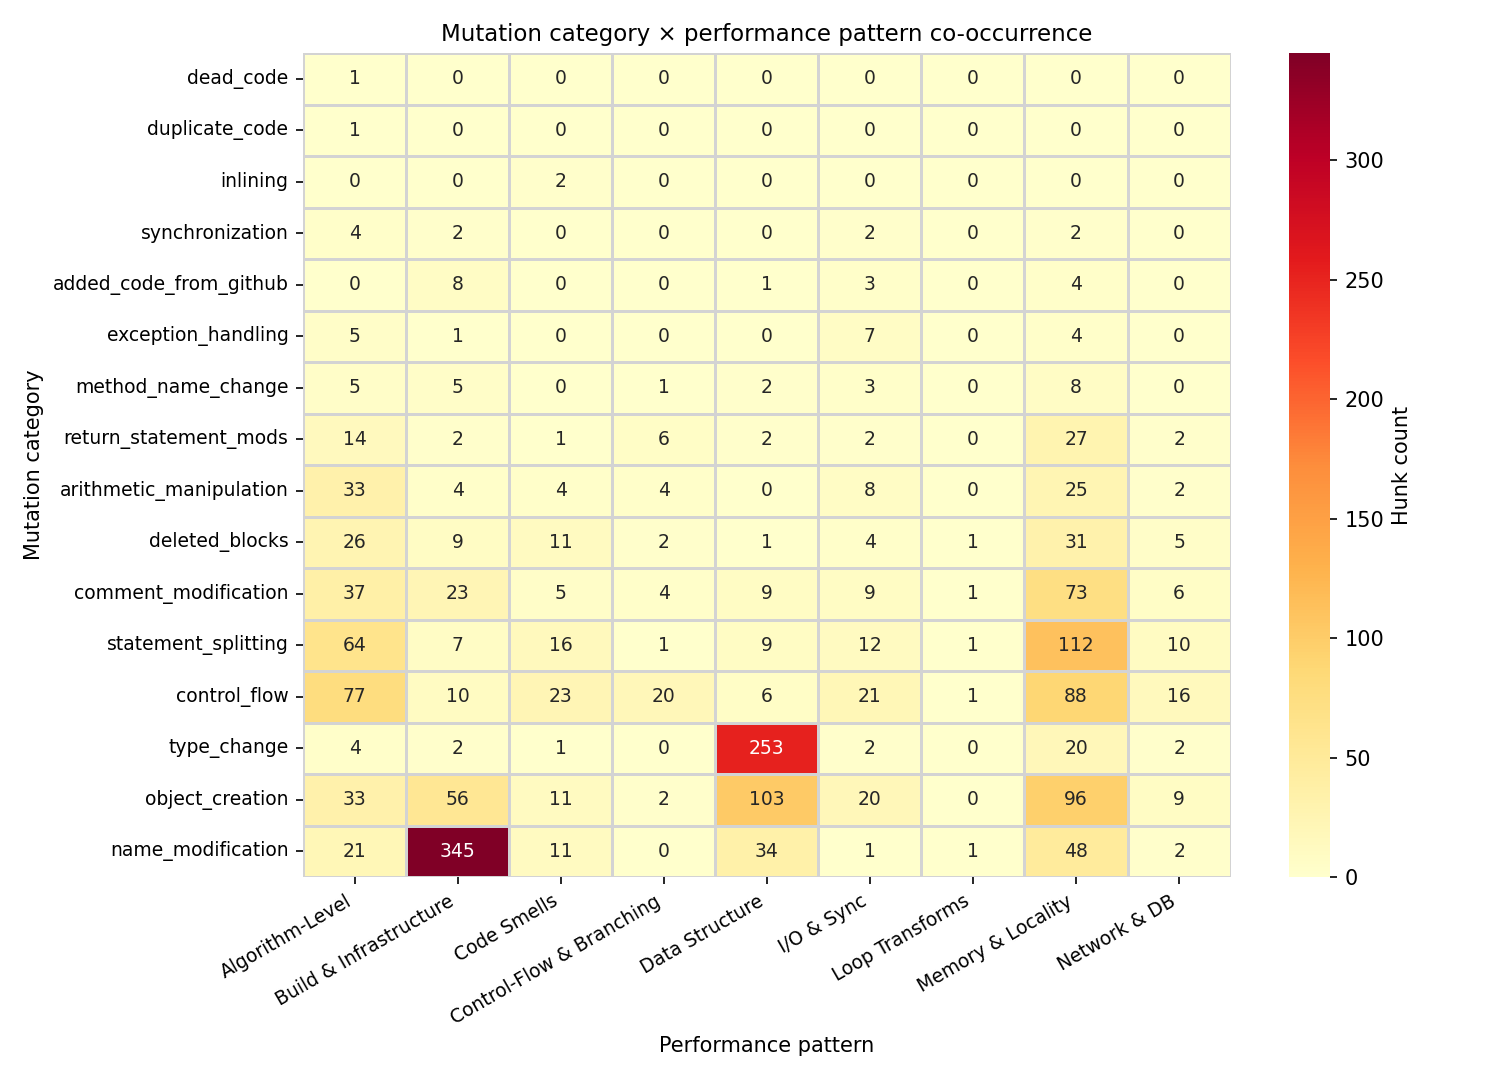
\includegraphics[height=0.8\textheight]{figs/heatmap_cat_pattern.png}
  \end{center}
\end{frame}

%---------------------------------------------------------
\begin{frame}{RQ2: Agent Mutation Vocabularies}
  Different agents have distinct mutation signatures:
  \begin{itemize}
    \item \textbf{Devin}: Dominated by \emph{name\_modification} (54\%) (dependency swapping).
    \item \textbf{GitHub Copilot}: Led by \emph{type\_change} (38\%) (data-structure upgrades).
    \item \textbf{OpenAI Codex}: Broadest structural profile; led by \emph{control\_flow} (24\%) and \emph{object\_creation} (18\%).
    \item \textbf{Cursor}: Elevated \emph{comment\_modification} (22\%) (adds explanatory annotations alongside diffs).
  \end{itemize}
\end{frame}

%---------------------------------------------------------
\begin{frame}{Agent Mutation Profiles Table}
  \begin{table}
    \centering\footnotesize
    \begin{tabular}{lrrrr}
      \toprule
      \textbf{Category} & \textbf{Devin} & \textbf{Copilot} & \textbf{Codex} & \textbf{Cursor} \\
      \midrule
      name\_modification    & \textbf{361} &  30 &  61 & 11 \\
      object\_creation      &  81 & 116 & 101 & 29 \\
      type\_change          &  35 & \textbf{224} &  22 &  2 \\
      control\_flow         &  51 &  48 & \textbf{136} & 24 \\
      statement\_splitting  &  65 &  49 &  95 & 21 \\
      comment\_modification &  22 &  64 &  37 & \textbf{41} \\
      \midrule
      \textit{All categories (total)} & \textit{670} & \textit{591} & \textit{574} & \textit{184} \\
      \bottomrule
    \end{tabular}
    \caption{Top mutation categories by agent (counts from 1,254 hunks).}
  \end{table}
\end{frame}

%---------------------------------------------------------
\begin{frame}{Implications for SBSE \& GI}
  \begin{block}{Priors for Reducing Search Space}
    By conditioning mutation operators on \textbf{agent identity} and \textbf{target optimization strategy}, we narrow the search space from 18 categories to a small handful.
  \end{block}
  
  \begin{itemize}
    \item \textbf{Example 1}: Optimizing Data Structures? Limit operators to \emph{type\_change} and \emph{object\_creation}.
    \item \textbf{Example 2}: Optimizing Build/Infra? Focus on \emph{name\_modification} (dependency substitutions).
    \item Directly increases search efficiency in agent-assisted GI.
  \end{itemize}
\end{frame}

\begin{frame}{Threats to Validity \& Limitations}
  \begin{itemize}
    \item \textbf{Language Confound}: Agent and target language are correlated in the dataset (Devin $\rightarrow$ TypeScript, Copilot $\rightarrow$ Rust, Codex $\rightarrow$ Go); signatures reflect a mix of agent style and ecosystem.
    \item \textbf{Taxonomy Scope}: Extended \emph{object\_creation} to include module-level imports, explaining its high rate (26.4\%) compared to traditional Java method-level scope.
    \item \textbf{Merged vs. Unmerged}: Includes both merged (324 hunks) and unmerged (927 hunks). Top categories overlap strongly ($\rho = 0.90$), but \emph{control\_flow} and \emph{statement\_splitting} are $\sim$3$\times$ more prevalent in merged hunks.
    \item \textbf{Judge Limitations}: LLM accuracy is bounded ($\sim$67.5\%); using the intersection strategy ensures conservative lower bounds.
  \end{itemize}
\end{frame}

%---------------------------------------------------------
\begin{frame}{Conclusion}
  \begin{itemize}
    \item \textbf{Legibility}: Opaque AI agent contributions can be reverse-engineered using SBSE mutation theory.
    \item \textbf{Structural Specificity}: Agent performance PRs focus on name modifications, object creations, and type changes—unlike traditional GI's flat distributions.
    \item \textbf{Empirical Priors}: Context-aware operator selection (knowing the agent and optimization target) drastically reduces the SBSE mutation space.
  \end{itemize}
\end{frame}

\end{document}
